% Class Notes Template
\documentclass[12pt]{article}
\usepackage[margin=1in]{geometry} 
\usepackage[utf8]{inputenc}

% Packages
\usepackage[french, english]{babel}
\usepackage{amsmath, amsthm, amssymb ,amsfonts, graphics, tikz, float, enumerate}
\usepackage{listings}
\usepackage{color} %red, green, blue, yellow, cyan, magenta, black, white
\definecolor{mygreen}{RGB}{28,172,0} % color values Red, Green, Blue
\definecolor{mylilas}{RGB}{170,55,241}

\lstset{language=Matlab,%
	%basicstyle=\color{red},
	breaklines=true,%
	morekeywords={matlab2tikz},
	keywordstyle=\color{blue},%
	morekeywords=[2]{1}, keywordstyle=[2]{\color{black}},
	identifierstyle=\color{black},%
	stringstyle=\color{mylilas},
	commentstyle=\color{mygreen},%
	showstringspaces=false,%without this there will be a symbol in the places where there is a space
	numbers=left,%
	numberstyle={\tiny \color{black}},% size of the numbers
	numbersep=9pt, % this defines how far the numbers are from the text
	emph=[1]{for,end,break},emphstyle=[1]\color{blue}, %some words to emphasise
	%emph=[2]{word1,word2}, emphstyle=[2]{style},    
}

% Title
\title{ECON 6130 - Problem Set \# 3}
\date{\today}
\author{Julien Manuel Neves}

% Use these for theorems, lemmas, proofs, etc.
\theoremstyle{definition}
\newtheorem{example}{Example}[section]
\newtheorem{theorem}{Theorem}
\newtheorem{lemma}[theorem]{Lemma}
\newtheorem{proposition}[theorem]{Proposition}
\newtheorem{claim}[theorem]{Claim}
\newtheorem{axiom}[theorem]{Axiom}
\newtheorem{corollary}[theorem]{Corollary}
\newtheorem{remark}[theorem]{Remark}
\newtheorem{definition}[theorem]{Definition}

% Usefuls Macros
\newcommand\N{\mathbb{N}}
\newcommand\E{\mathbb{E}}
\newcommand\R{\mathbb{R}}
\newcommand\F{\mathcal{F}}
\newcommand\Z{\mathbb{Z}}
\newcommand\st{\text{ such that }}
\newcommand\seq[1]{\{ #1 \}}
\newcommand{\inv}{^{-1}}

\newcommand{\pa}[1]{\left(#1\right)}
\newcommand{\bra}[1]{\left[#1\right]}
\newcommand{\cbra}[1]{\left\{#1\right\}}

\newcommand{\pfrac}[2]{\pa{\frac{#1}{#2}}}
\newcommand{\bfrac}[2]{\bra{\frac{#1}{#2}}}

\newcommand{\mat}[1]{\begin{matrix}#1\end{matrix}}
\newcommand{\pmat}[1]{\pa{\mat{#1}}}
\newcommand{\bmat}[1]{\bra{\mat{#1}}}


\begin{document}

\maketitle

\section*{Problem 1}
\subsection*{1.}
\begin{figure}[H]
	\centering
	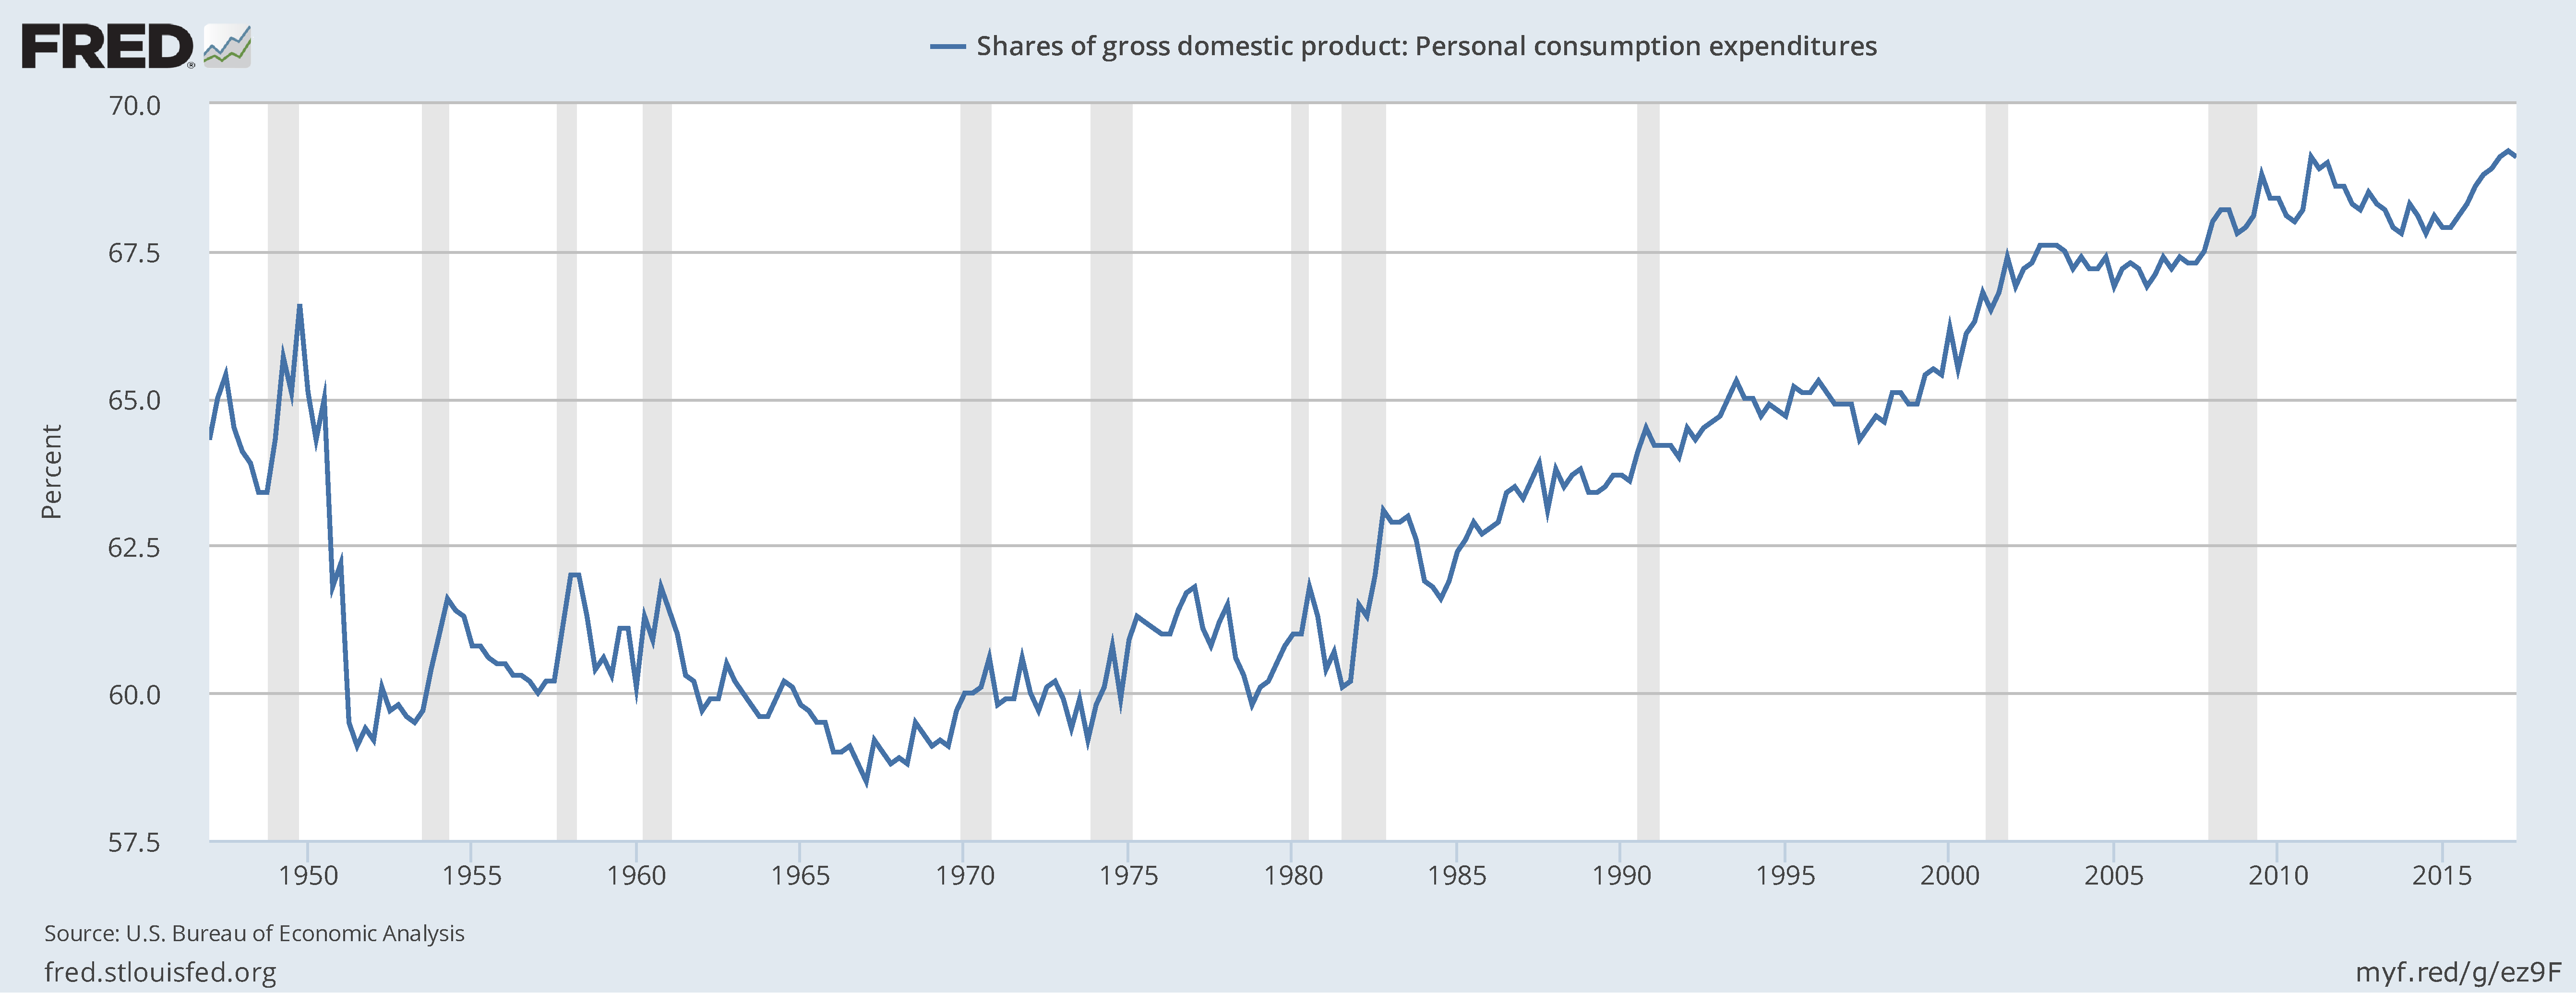
\includegraphics[width=0.9\linewidth]{plot1}
	\label{fig:plot1}
\end{figure}

\begin{enumerate}[(i)]
	\item On average 65\% and closer to 68\% in the last few years.
	\item Stationary.
	\item Trending upward. Accordingly, it steadily increased by roughly 10\% over the course of the last 50 years.
	\item Small and rapid fluctuations around the trend, (less than 1\%).
	\item Stable even during the recessions.
\end{enumerate}

\subsection*{2.}
\begin{figure}[H]
	\centering
	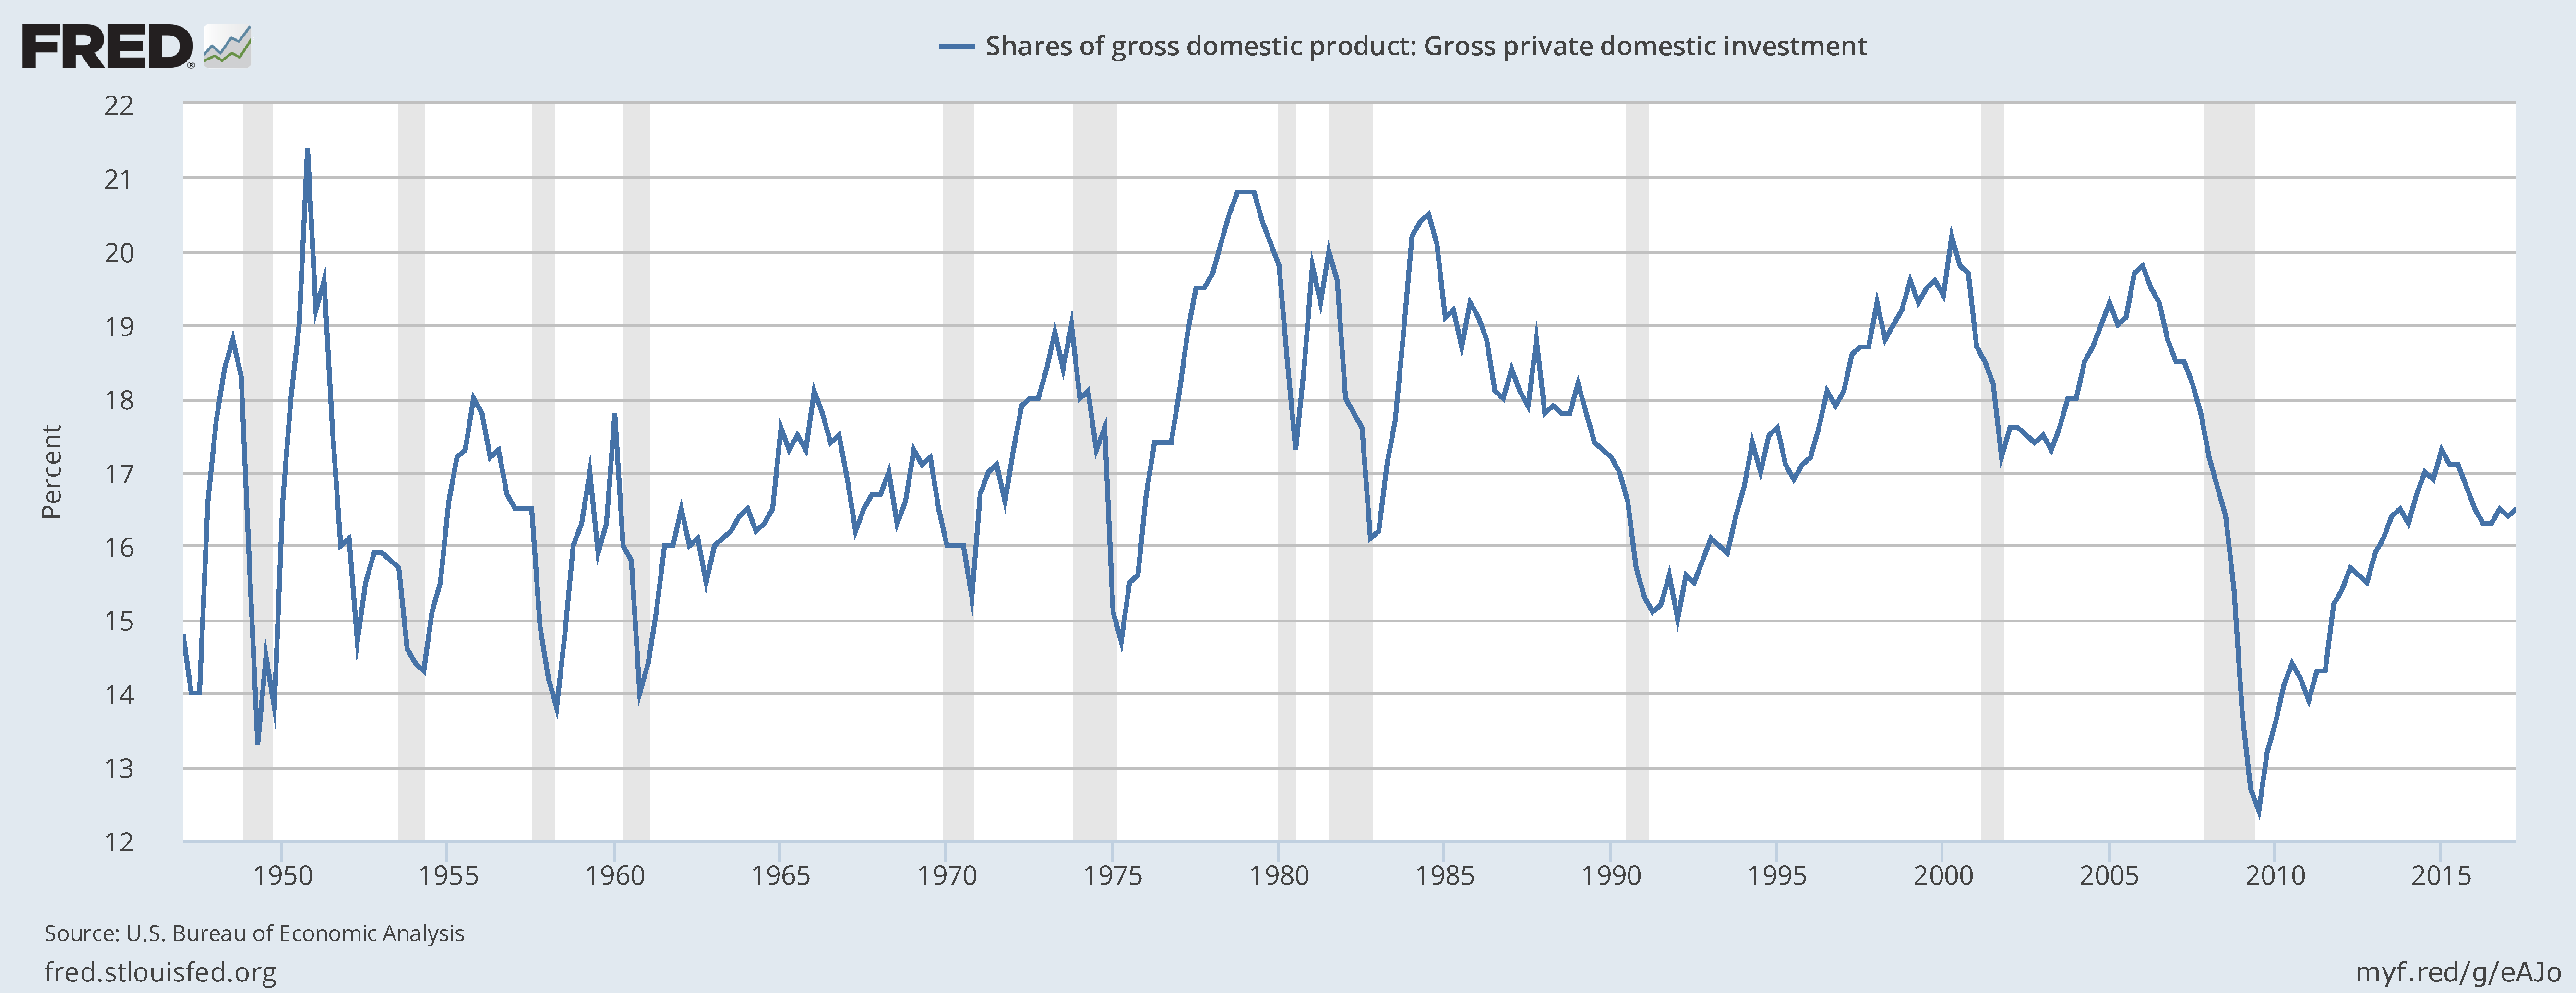
\includegraphics[width=0.9\linewidth]{plot2}
	\label{fig:plot2}
\end{figure}

\begin{enumerate}[(i)]
	\item On average 17\%.
	\item Stationary.
	\item No trend. It fluctuates around its mean.
	\item Big and rapid fluctuations around the trend (up to 8\%). This contrasts with consumption.
	\item Investment seem to drop enormously during recessions. Again, this is in opposition to the previous figure.
\end{enumerate}

\subsection*{3.}
\begin{figure}[H]
	\centering
	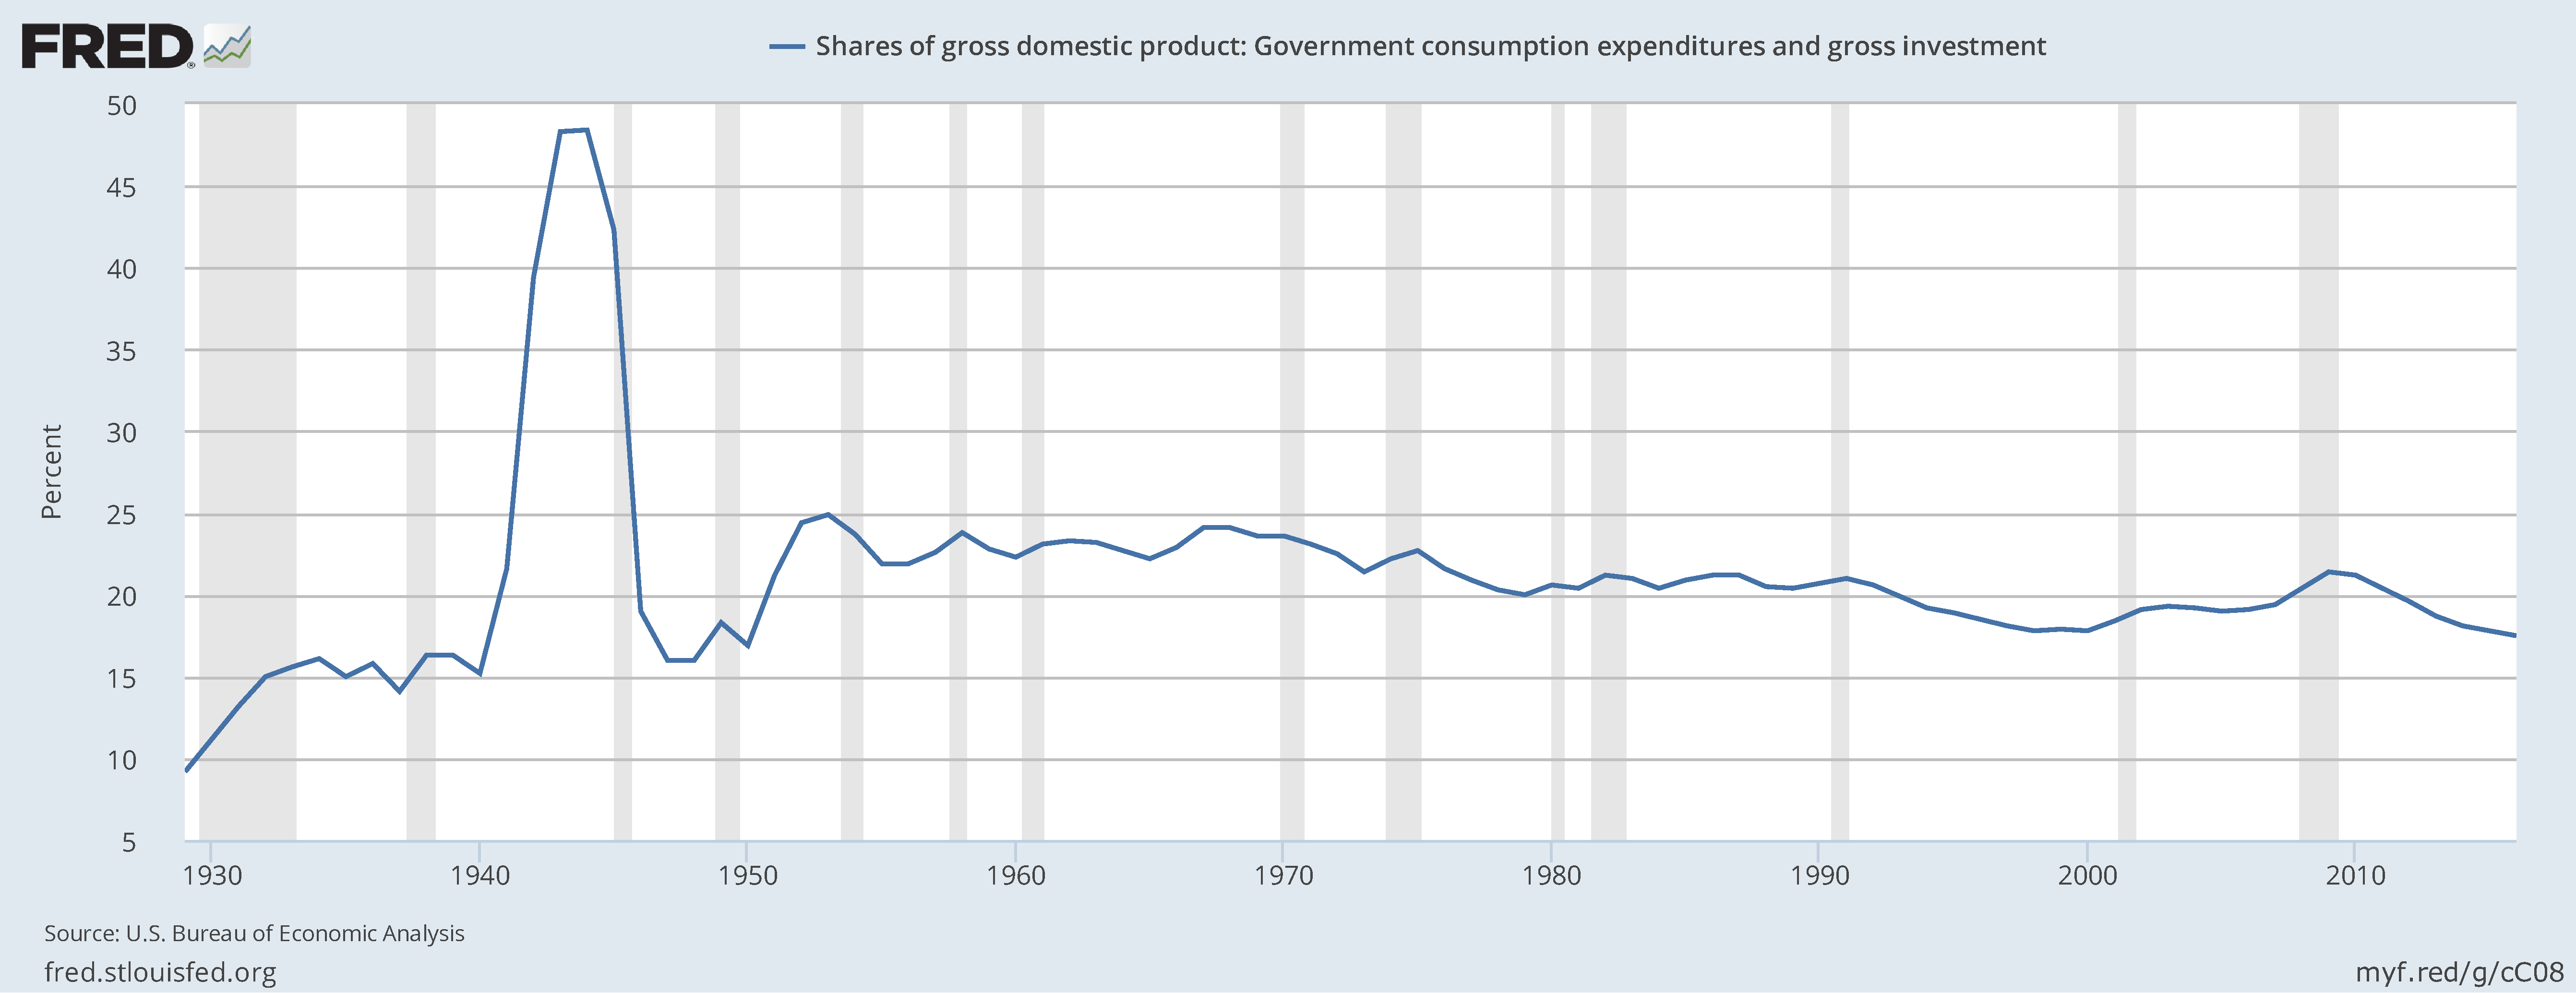
\includegraphics[width=0.9\linewidth]{plot3}
	\label{fig:plot3}
\end{figure}

\begin{enumerate}[(i)]
	\item On average 20\%.
	\item Stationary.
	\item No trend. It fluctuates around its mean.
	\item Really smooth curve around the trend after World War II. This comes from the fact that plans for government spending are usually adopted once a year. Moreover, the increase during World War II comes from the major military spending the U.S. government incurred during that period.
	\item Slightly increasing during recessions.
\end{enumerate}

\subsection*{4.}
\begin{figure}[H]
	\centering
	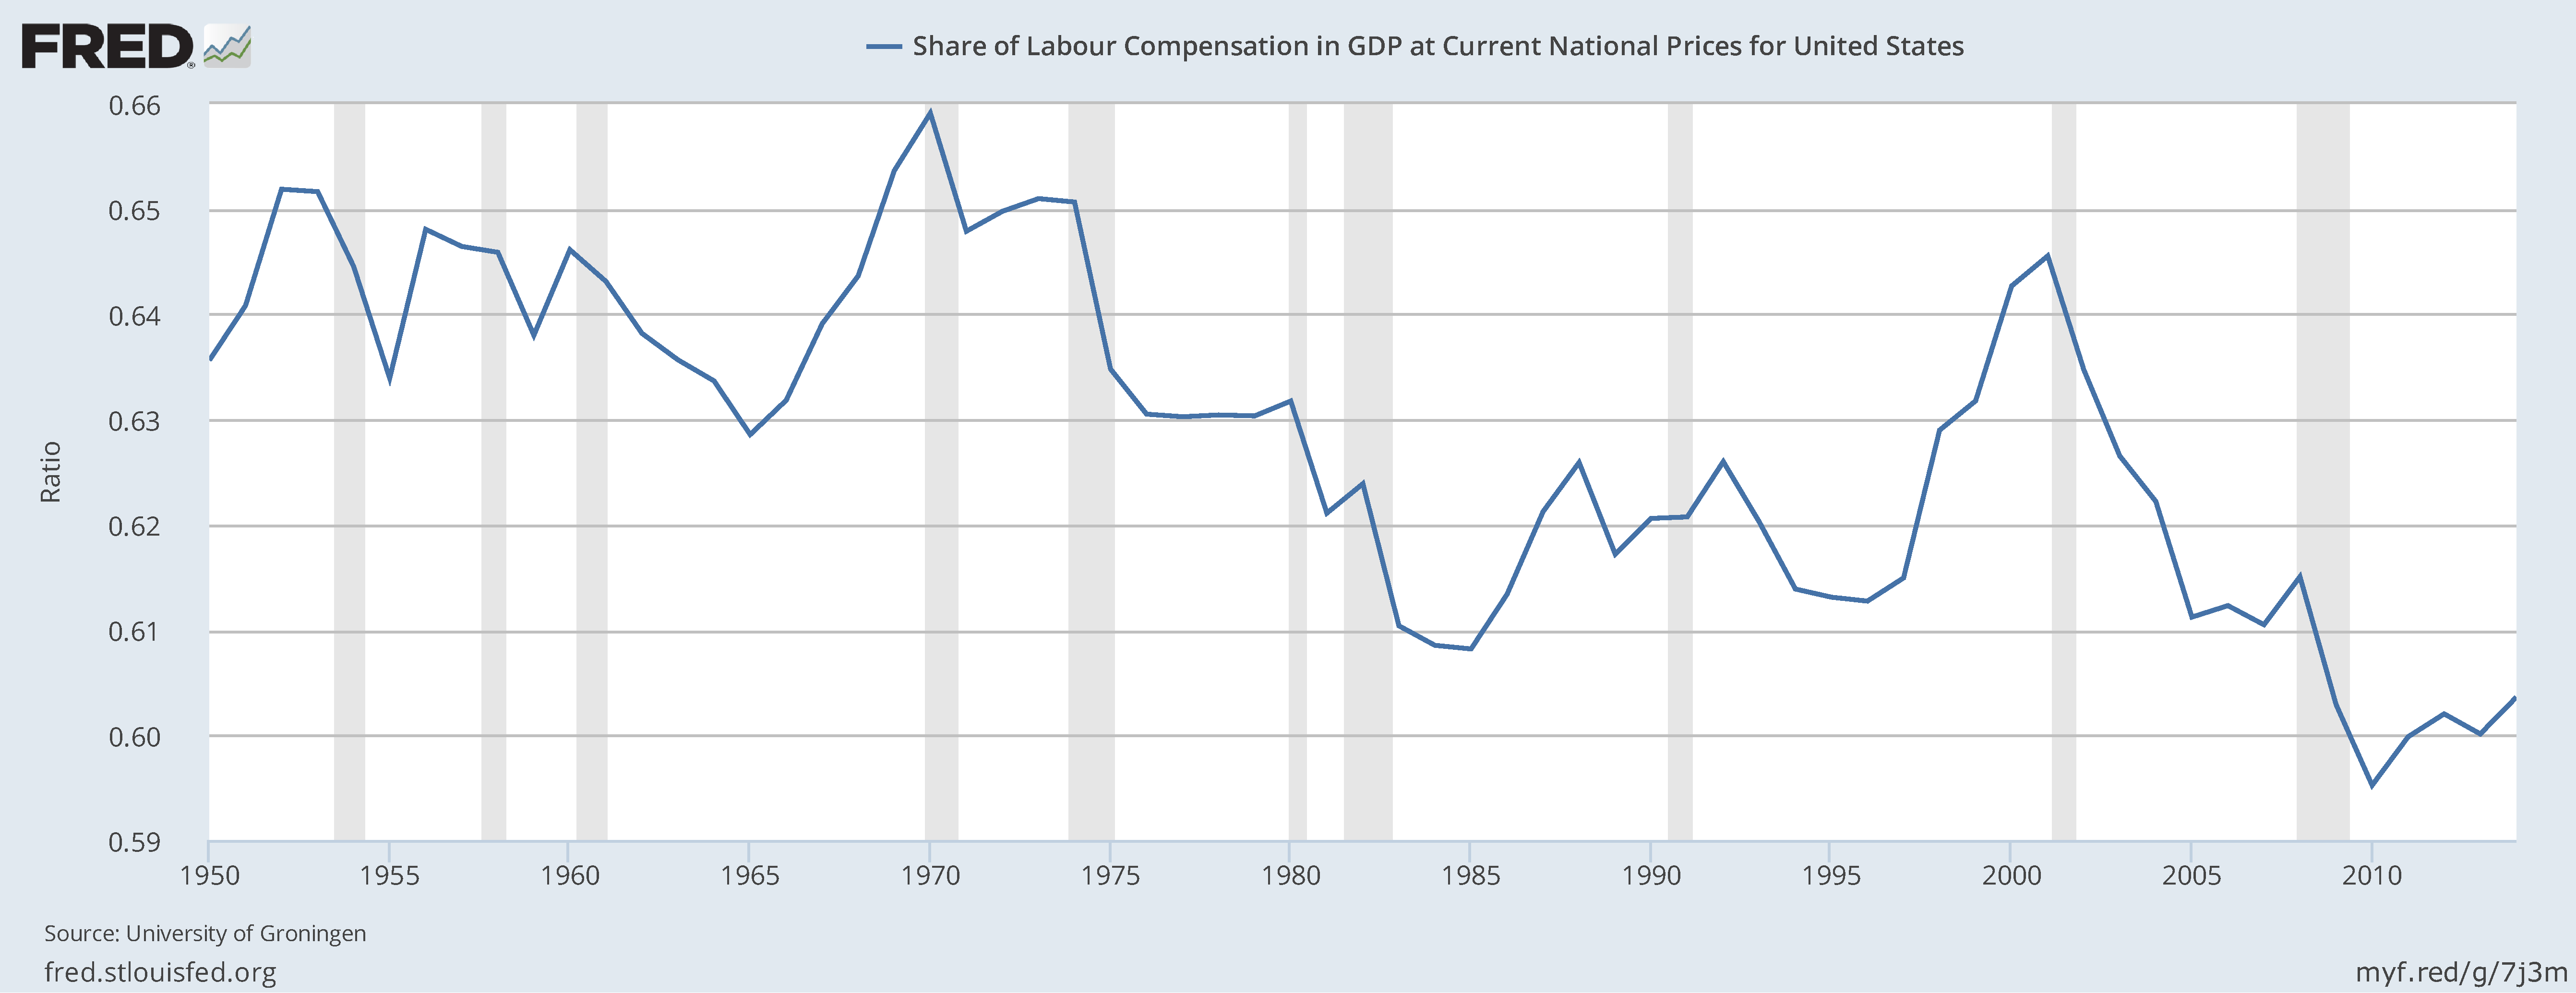
\includegraphics[width=0.9\linewidth]{plot4}
	\label{fig:plot4}
\end{figure}

\begin{enumerate}[(i)]
	\item On average 63\%.
	\item Stationary.
	\item Stable before 1975 and slightly declining after 1975 (drop by roughly 6\% over the course of the last 30 years).
	\item Small and slow fluctuations around the trend (around 1\%).
	\item Sharp declines during recessions. In the recent one, payments to labor as share of GDP drop by 2\%.
\end{enumerate}

\subsection*{5.}

Note this figure was constructed by taking the complement of the previous series.
\begin{figure}[H]
	\centering
	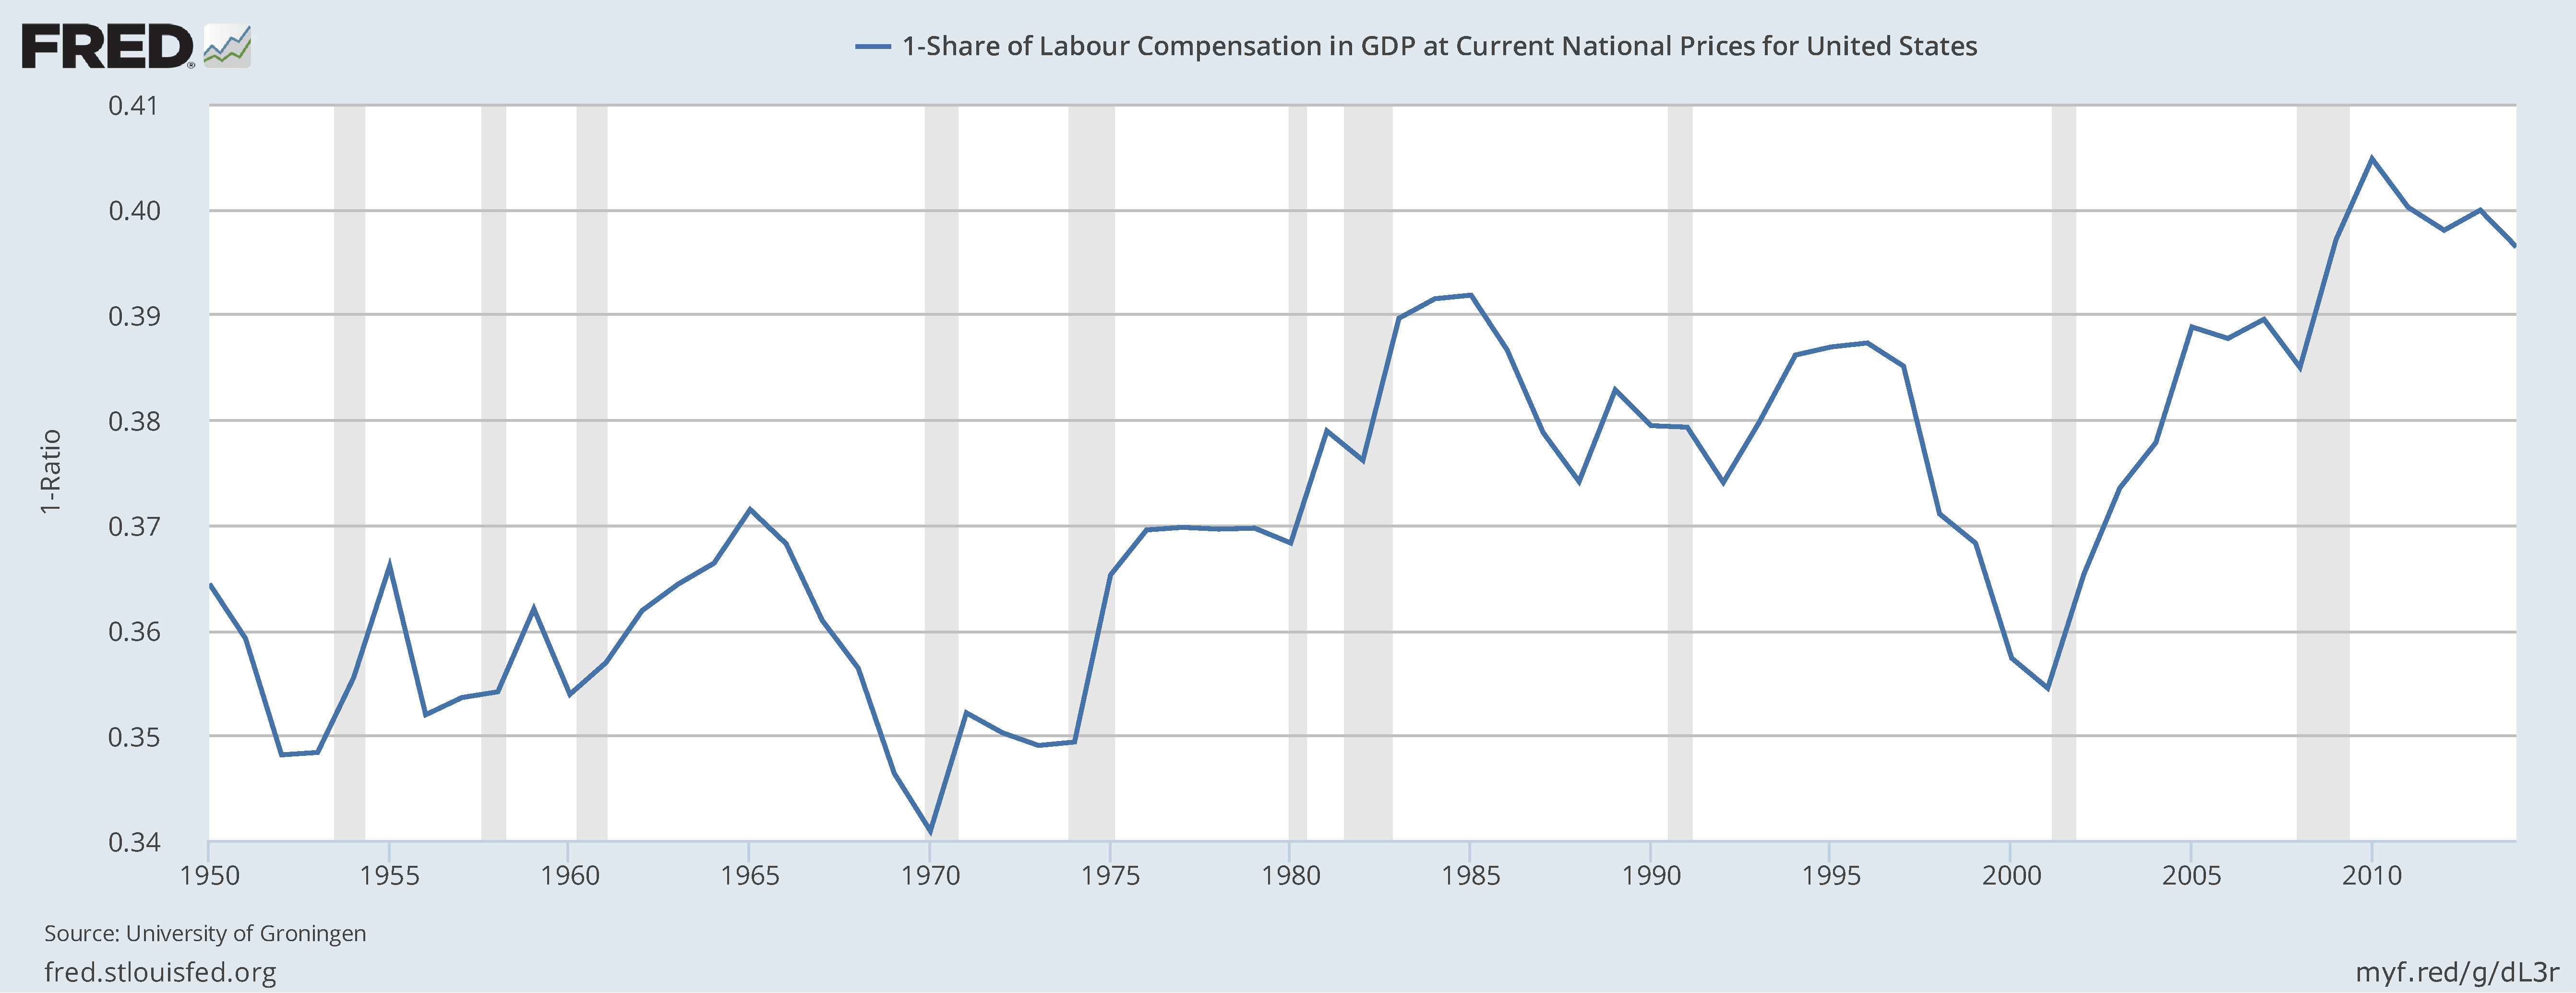
\includegraphics[width=0.9\linewidth]{plot5}
	\label{fig:plot5}
\end{figure}

\begin{enumerate}[(i)]
	\item On average 37\%.
	\item Stationary.
	\item Stable before 1975 and slightly increasing after 1975 (drop by roughly 6\% over the course of the last 30 years).
	\item Small and slow fluctuations around the trend (around 1\%).
	\item Sharp increases during recessions. In the recent one, payments to capital as share of GDP jump by 2\%.
\end{enumerate}

\subsection*{6.}
\begin{figure}[H]
	\centering
	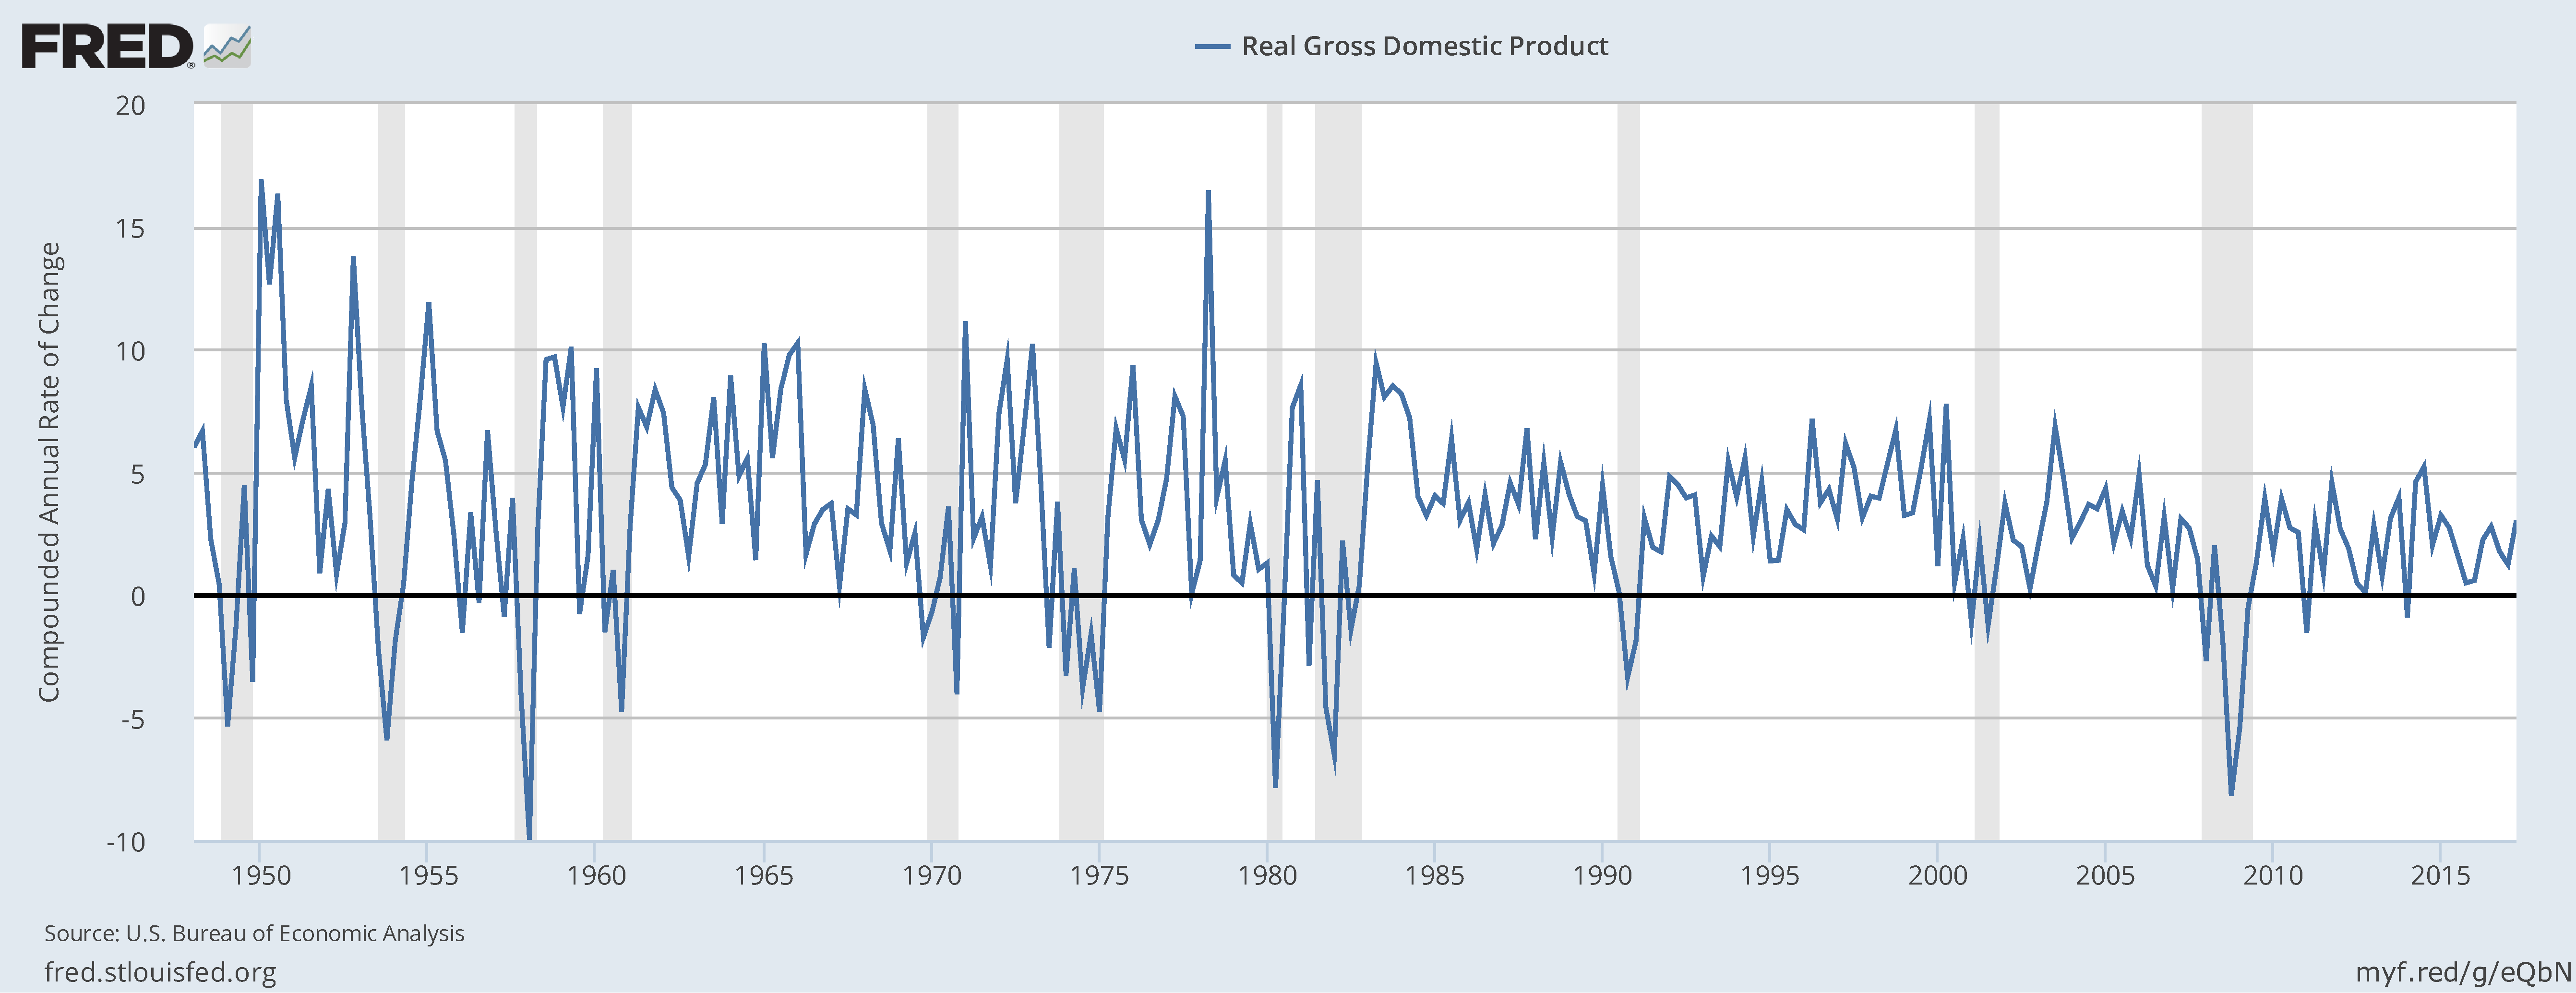
\includegraphics[width=0.9\linewidth]{plot6}
	\label{fig:plot6}
\end{figure}

\begin{enumerate}[(i)]
	\item On average 2-3 \%.
	\item Stationary.
	\item Stable around the mean.
	\item Rapid and large fluctuations around the trend (around 5\%). More volatile before 1980.
	\item Sharp decline during the recessions. In the recent recession, $\hat{Y}_i$ drop by 8\%.
\end{enumerate}

\subsection*{7.}
\begin{figure}[H]
	\centering
	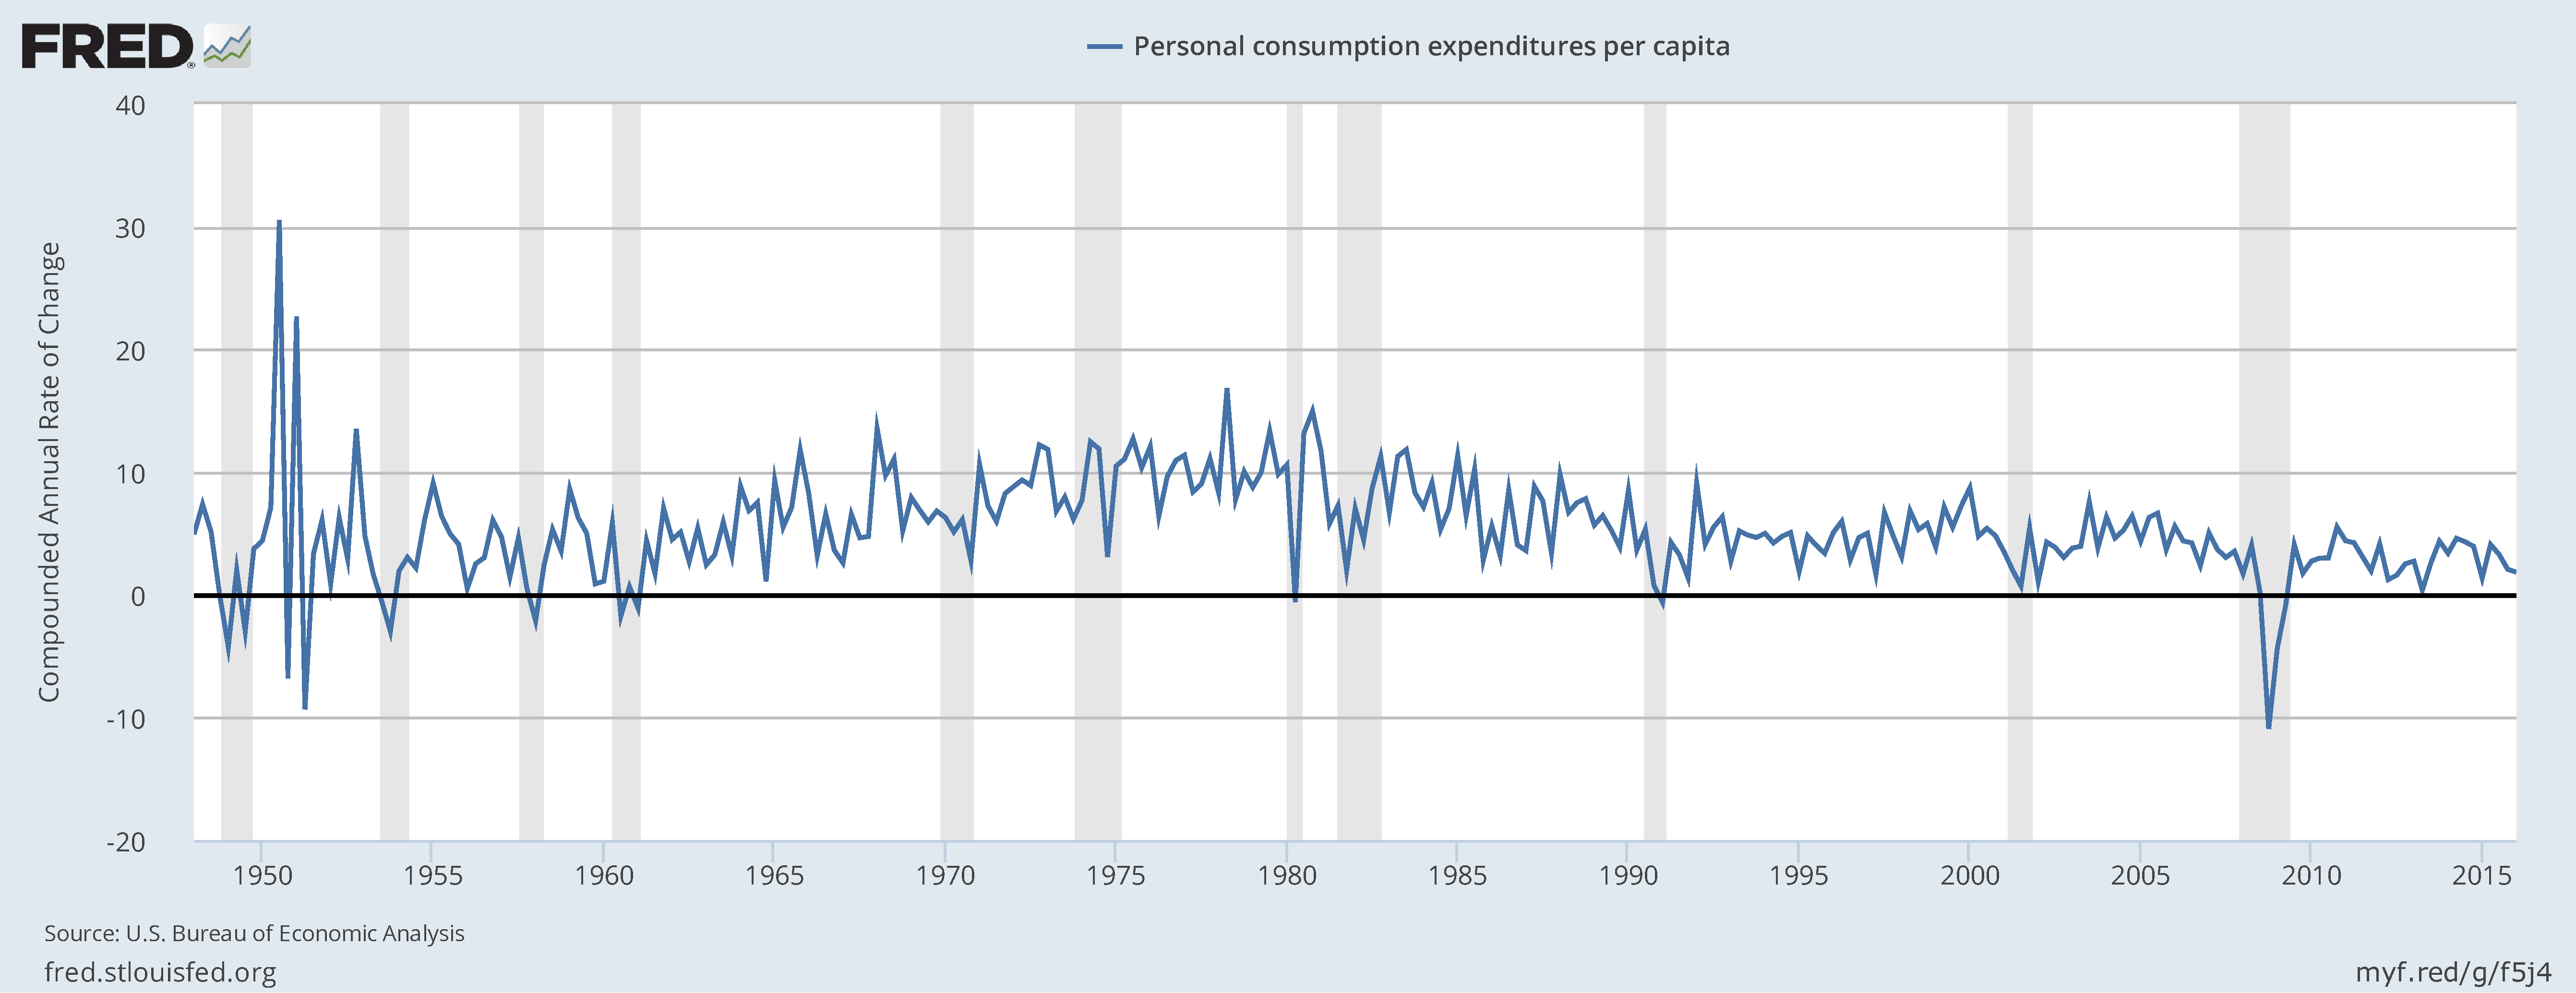
\includegraphics[width=0.9\linewidth]{plot7}
	\label{fig:plot7}
\end{figure}

\begin{enumerate}[(i)]
	\item On average 3 \%.
	\item Stationary.
	\item Stable around the mean.
	\item Rapid and small fluctuations around the trend (around 2\%). More volatile before 1955.
	\item Sharp decline during the recessions. In the recent recession, $\hat{c}_i$ drop by 8\%.
	\item Follows the growth rate of GDP pretty closely.
\end{enumerate}


\subsection*{8.}
\begin{figure}[H]
	\centering
	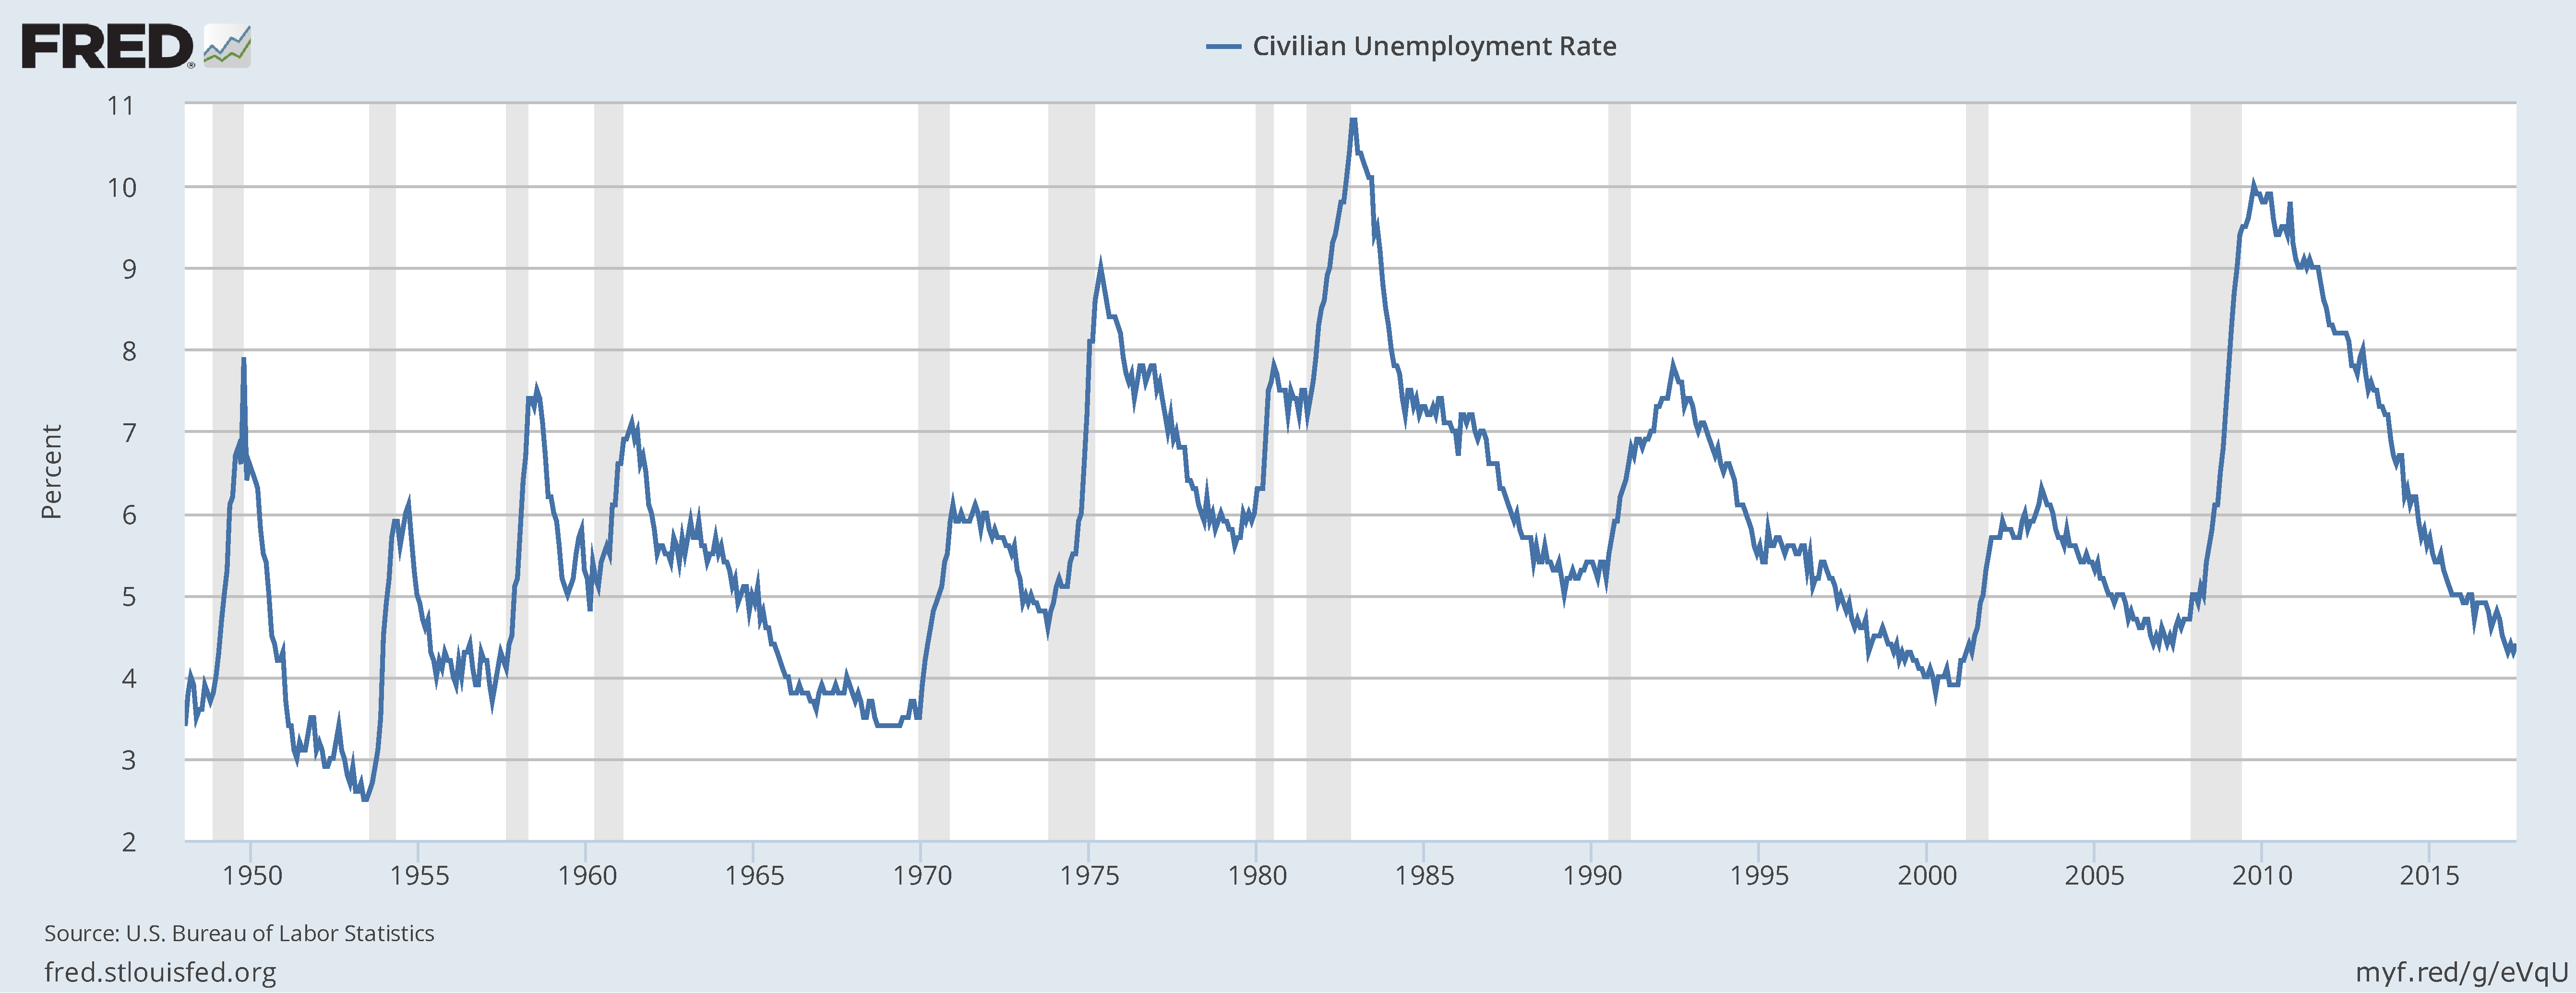
\includegraphics[width=0.9\linewidth]{plot8}
	\label{fig:plot8}
\end{figure}

\begin{enumerate}[(i)]
	\item On average 6 \%.
	\item Stationary.
	\item Overall trend: sharp increase during the recessions followed by slow recovery.
	\item Small fluctuation around overall trend.
	\item In recent recession, unemployment went up by around 6\% and only just now is it back to its original level.
\end{enumerate}

\subsection*{9.}
\begin{figure}[H]
	\centering
	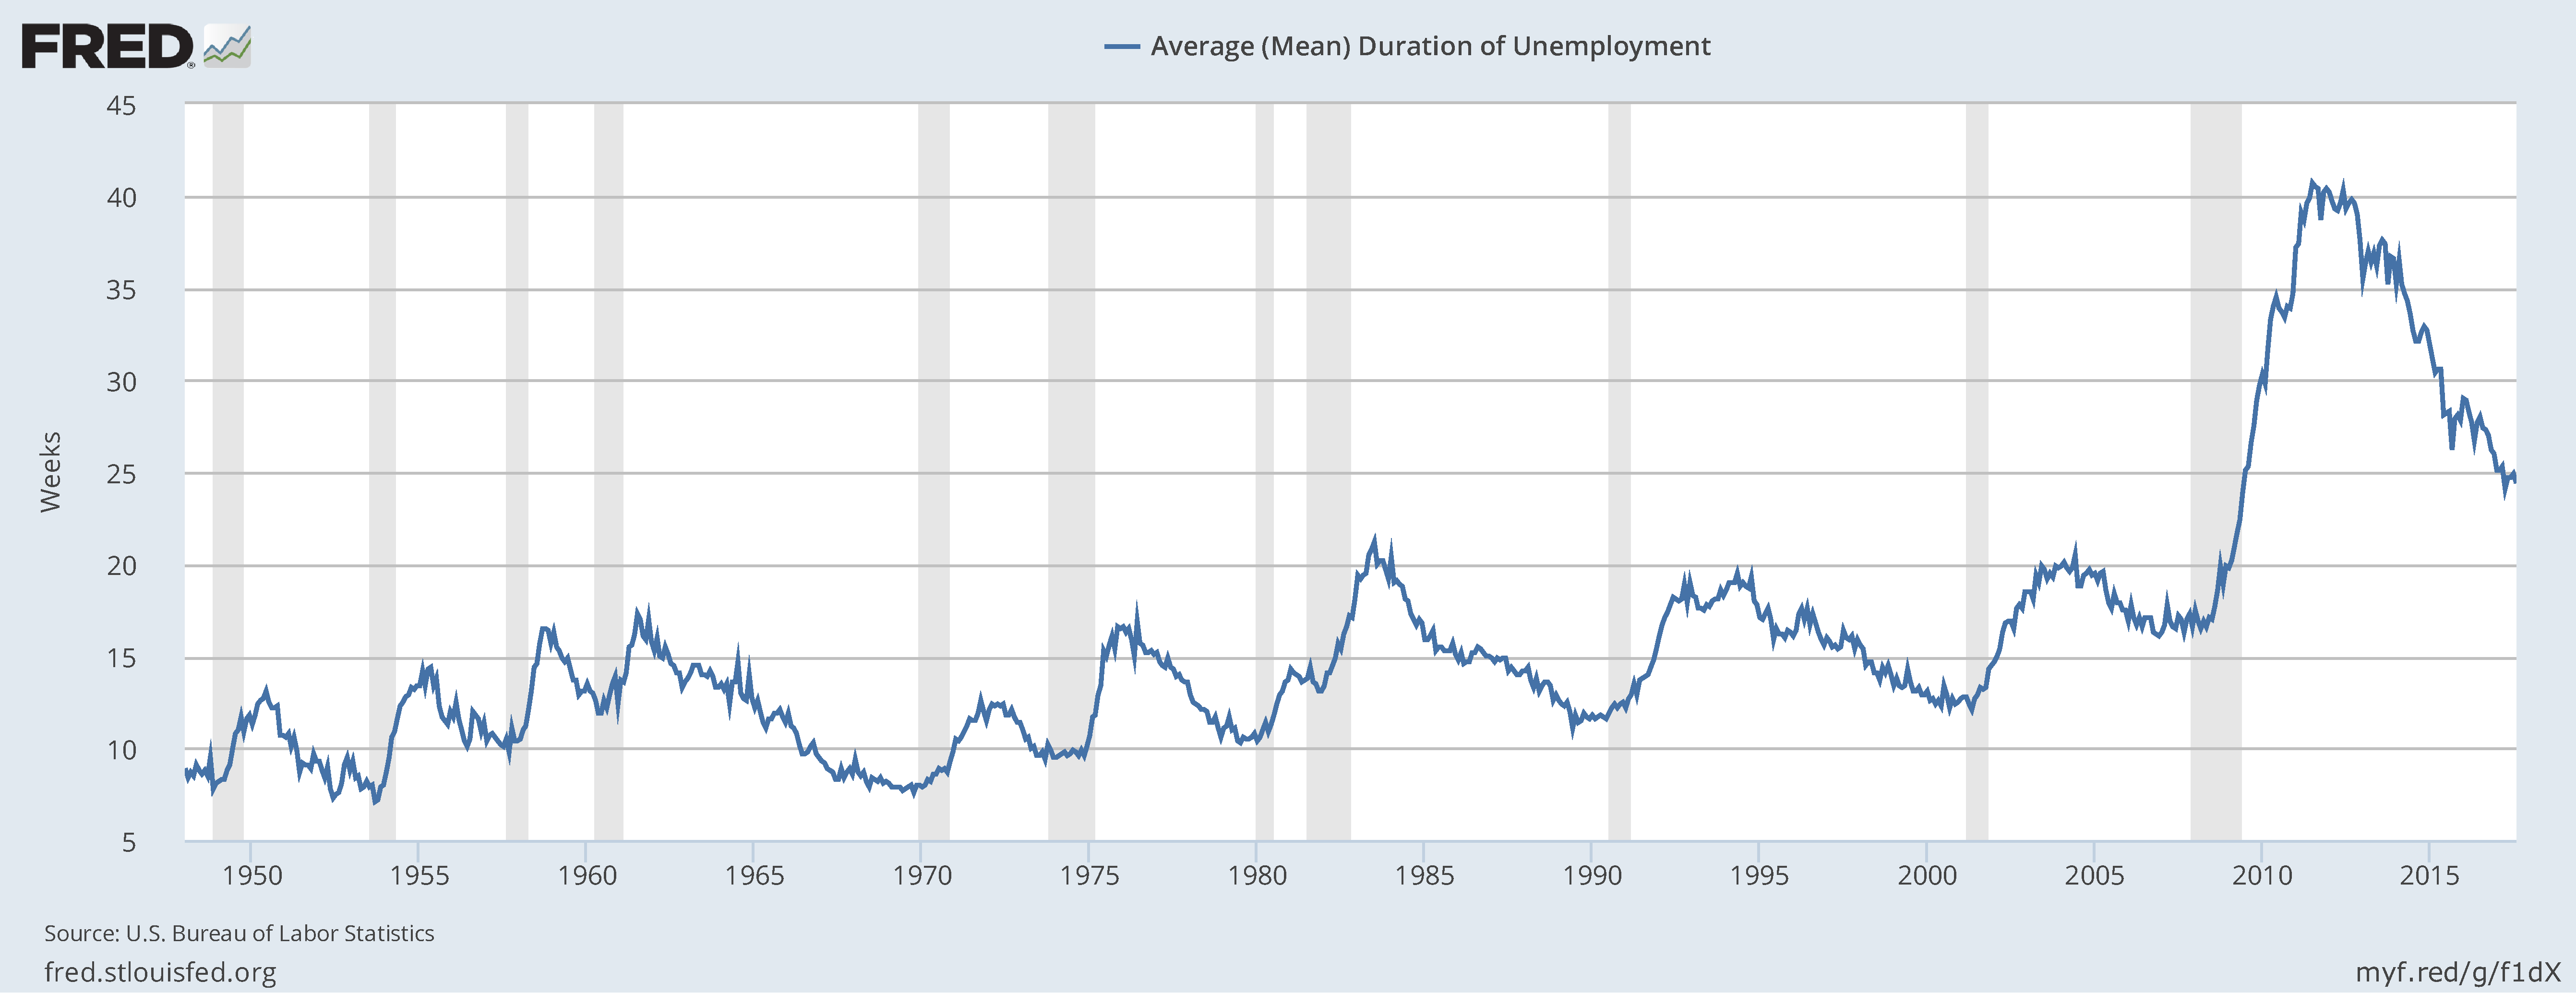
\includegraphics[width=0.9\linewidth]{plot9}
	\label{fig:plot9}
\end{figure}

\begin{enumerate}[(i)]
	\item On average 13 weeks before 2000 and 30-35 weeks in the last decade.
	\item Non-stationary.
	\item Overall trend: sharp increase during the recessions followed by slow recovery. Unlike the unemployment rate, the support for the average duration of unemployment seems to be increasing at an exponential rate.
	\item Small fluctuations around the trend. 
	\item In recent recession, average duration increase up to 40 weeks and is only just now back to 25 weeks. This contrast with previous recessions where average duration would consistently increase to roughly 15 weeks and go back down to 10 weeks afterwards.
\end{enumerate}


\section*{Problem 2}

\subsection*{1.}

Planner's optimization problem:
\begin{align*}
	v(k)=&\max_{ 0\leq k'\leq f(k)}\left\lbrace   \log(f(k)-k') +\beta v(k')\right\rbrace
\end{align*}
where $f(k)=F(k,1)+(1-\delta)k = k^\alpha + (1-\delta)k$.

For simplicity, this problem can be reformulated as such
\begin{align*}
v(k)=&\max_{ 0\leq k'\leq k^\alpha + (1-\delta)k}\left\lbrace   \log(k^\alpha + (1-\delta)k-k') +\beta v(k') \right\rbrace
\end{align*}
where
\begin{enumerate}[(i)]
	\item State Variable $\Rightarrow k$.
	
	We can interpret $k$ as the level of capital today. For the planner, it is taken as given, and its value influence the state of the world. In the setting of this problem, $k$ constrains the amount of goods available today by $f(k)$.
	\item Control Variable $\Rightarrow k'$.
	
	While the planner is constraint by the current level of capital, he is free to choose the level of capital in the next period, i.e. $k'$. In this problem, the planner is maximizing today's utility and tomorrow's future value of utility by setting $k'$.
\end{enumerate}

Note that in this dynamic setting there's no need for an aggregate law of motion for the state variables since the planner is already at the aggregate level.

\subsection*{2.}

Note that instead of looking at a large grid, we can narrow our search by first finding the steady state, i.e. $k=k_t=k_{t+1}$.

Using the Euler equation of the sequential problem we have
\begin{align*}
	u'(f(k_t)-k_{t+1})&=\beta u'(f(k_{t+1})-k_{t+2})f'(k_t)\\
	\frac{1}{f(k_t)-k_{t+1}}&=\beta \frac{1}{f(k_{t+1})-k_{t+2}}(\alpha k_t^{\alpha-1}+(1-\delta))\\
	\frac{1}{f(k)-k}&=\beta \frac{1}{f(k)-k}(\alpha k^{\alpha-1}+(1-\delta))\\
	\frac{1}{\beta}&=\alpha k^{\alpha-1}+(1-\delta)\\
	k&=\left[ \frac{1-\beta +\beta \delta}{\alpha\beta }\right]^{\frac{1}{{\alpha-1}}} \\
\end{align*}

Given $\alpha = 0.3$, $\beta = 0.6$ and $\delta=0.8$, then 
\begin{align*}
k&=\left[ \frac{1-\beta +\beta \delta}{\alpha\beta }\right]^{\frac{1}{{\alpha-1}}} \\
&=\left[ \frac{1-0.6 +0.6 \cdot 0.8}{0.3\cdot 0.6}\right]^{\frac{1}{{0.3-1}}}\\
& \approx 0.1036
\end{align*}

Thus, we can build a grid around $0.1036$ to capture the policy and value functions around the steady state.

With a grid of size $n=1000$, we have the following numerical solution:
\begin{figure}[H]
	\centering
	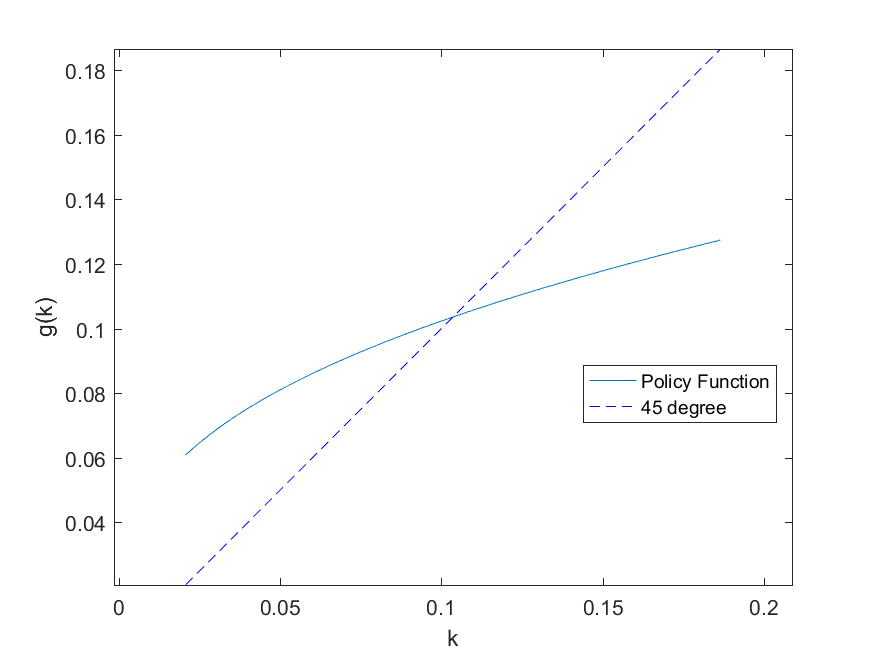
\includegraphics[width=0.8\linewidth]{plot_policy}
	\caption{Policy function}
	\label{fig:plotpolicy}
\end{figure}
\begin{figure}[H]
	\centering
	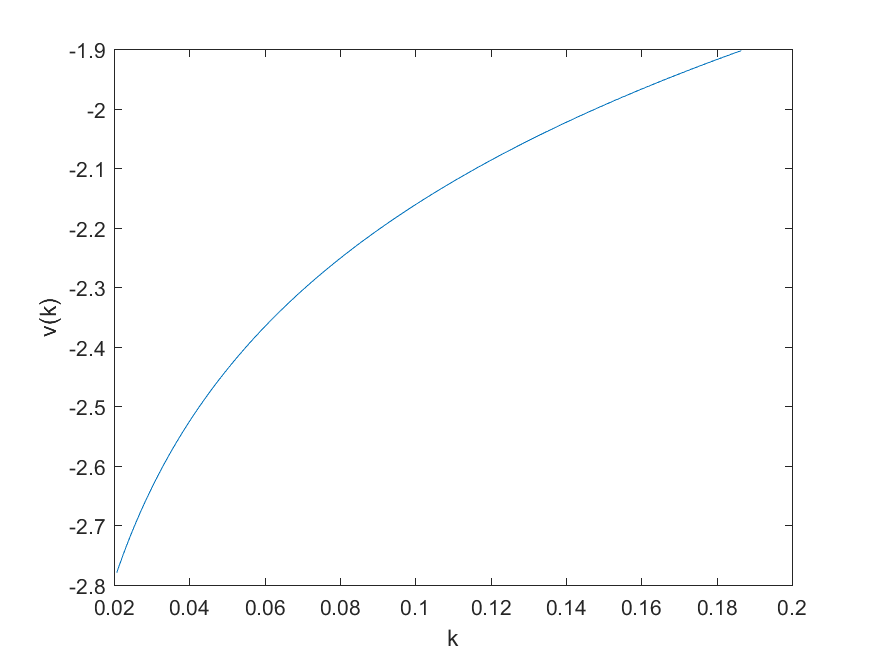
\includegraphics[width=0.8\linewidth]{plot_value}
	\caption{Value function}
	\label{fig:plotvalue}
\end{figure}


\lstinputlisting[language=Matlab]{value_function_ite.m}

\end{document}
